\section{系统实现}
\subsection{题库模块}
\begin{figure}[hb]
    \centering
    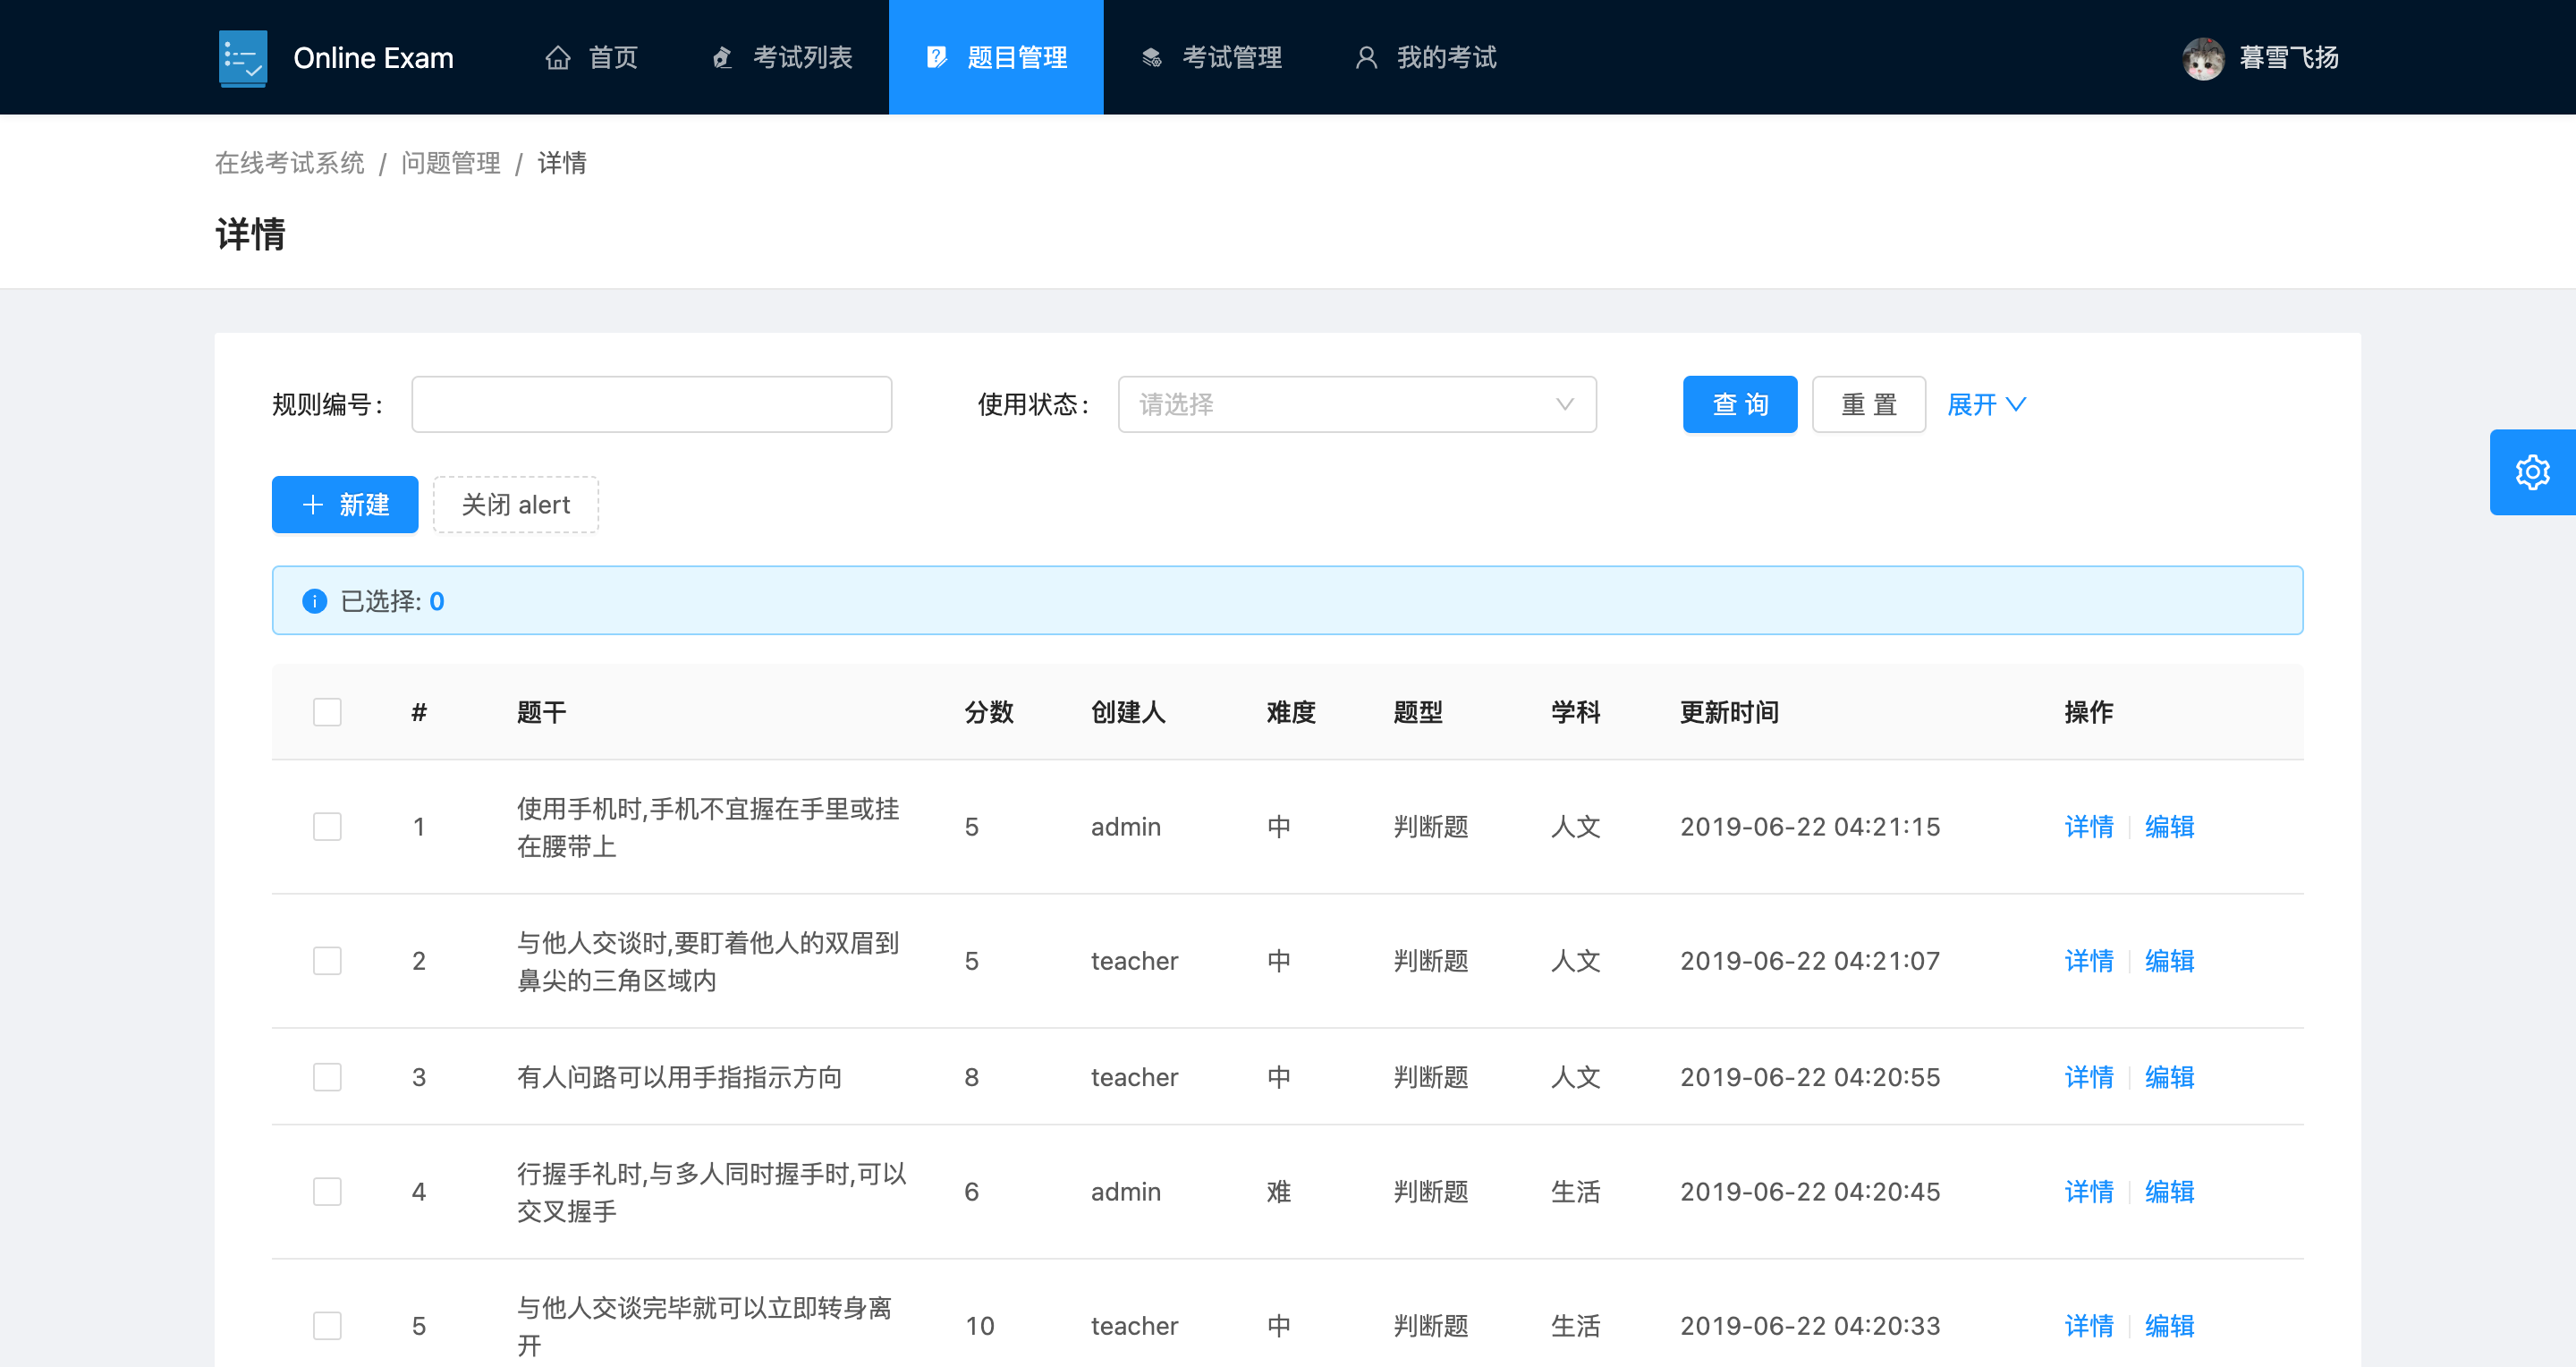
\includegraphics[width=\linewidth]{_images/题库模块截图.jpeg}
    \caption{题库模块}
\end{figure}
进入题库模块前需要先检查是否有进入的权限,如果没有则需要一定的 403 反馈。正常操作流程下,没有权限是无法通过点击事件进入题库,但也可能通过浏览器的地址栏 URL,通过路由器强行渲染出对应的题库 \lstinline!View! 组件,因此仍是需要在进入模块前进行权限检查。

如果有权限进入,则展示所有的题目,并可以进行分页操作、选择题库查看、选择具体题目操作。

分页操作,则需要在组件中托管具体的 \lstinline!current!、\lstinline!pageSize!、\lstinline!total! 数据,并注入 ant-d-v 提供的 \lstinline!<Pagination>!。分页请求时,向后端发起 \lstinline!/exam/question/list! 的 \lstinline!GET! 请求,并将 \lstinline!current! 和 \lstinline!pageSize! 作为参数。在后端 Controller 中接收请求,做处理。

\begin{lstlisting}[language=Java]
@GetMapping("/question/list")
@ApiOperation("获取问题的列表")
ResultVO<QuestionPageVo> getQuestionList(
    @RequestParam("pageNo") Integer pageNo, 
    @RequestParam("pageSize") Integer pageSize
) {
    ResultVO<QuestionPageVo> resultVO;
    
    try {
        QuestionPageVo questionPageVo = examService.getQuestionList(pageNo, pageSize);
        resultVO = new ResultVO<>(0, "获取问题列表成功", questionPageVo);
    } catch (Exception e) {
        e.printStackTrace();
        resultVO = new ResultVO<>(-1, "获取问题列表失败", null);
    }
    
    return resultVO;
}
\end{lstlisting}

选择具体题库,则展示具体题库下的题目。也可以进行修改题库信息、删除题库或新增题库。\upcite{ref12,ref14}

修改题库信息,可以修改题库的名称,或新增、删除其中包含的题目。

删除题库的操作,会将所有当前题库下的题目,与之解除关联。在具体的题库-题目 mapper 表中删除对应的映射。而不会删除具体的题目,即使已经没有任何题库与这些题目关联。但是这些题目仍是会在题库添加的时候,可选展示待加入。

新增题库的操作则会要求填写题库的基本信息,而后可以选择需要添加入题库的题目。也可以在创建成功以后,再通过修改题库的功能,对题库的题目做管理。

对于具体题目的操作,可以查看题目的详情,也可以对题目配置的属性做修改调整。

\begin{lstlisting}[language=Java]
@PostMapping("/question/update")
@ApiOperation("更新问题")
ResultVO<String> questionUpdate(@RequestBody QuestionVo questionVo) {
    // 完成问题的更新
    System.out.println(questionVo);
    try {
        examService.updateQuestion(questionVo);
        return new ResultVO<>(0, "更新问题成功", null);
    } catch (Exception e) {
        e.printStackTrace();
        return new ResultVO<>(-1, "更新问题失败", null);
    }
}
\end{lstlisting}

\begin{figure}[htb]
    \centering
    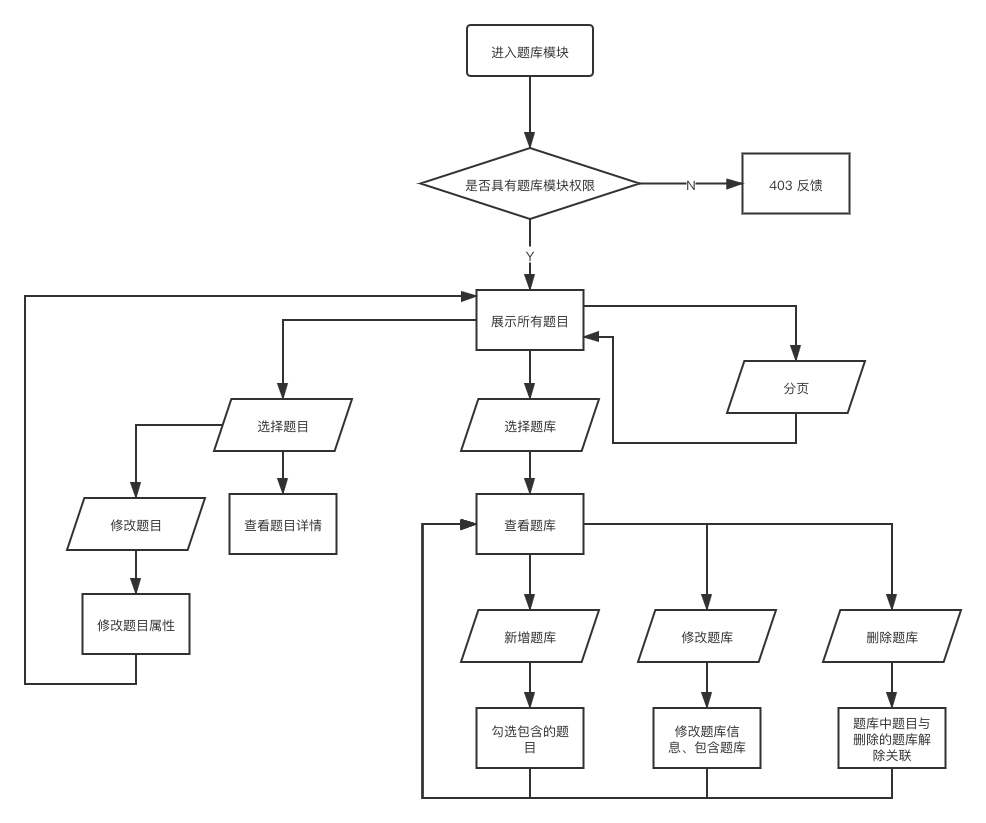
\includegraphics[width=\linewidth]{_images/题库模块.png}
    \caption{题库模块}
\end{figure}


\subsection{考卷模块}
进入考卷模块前需要先检查是否有进入的权限,如果没有则需要一定的 403 反馈。正常操作流程下,没有权限是无法通过点击事件进入考卷模块,但也可能通过浏览器的地址栏 URL,通过路由器强行渲染出对应的题库 \lstinline!View! 组件,因此仍是需要在进入考卷模块前进行权限检查。

\begin{lstlisting}[language=JavaScript]
export default {
  ... ...
  computed: {
      ... ...
      storeUserInfo: function(){
          return TokenManager.getToken().userInfo
      },
      ... ...
  },
  methods: {
      queryExamPaper: function(pageIndex){
          ... ...
          const userId = this.storeUserInfo?.id
          ... ...
          Requester.post(...)
          ... ...
      }
  },
  ... ...
}
\end{lstlisting}
如果有权限进入考卷模块,则需要从 store 中获取当前用户的 \lstinline!id!,并传入后端,并携带分页所需要的 \lstinline!current!、\lstinline!pageSize! 等信息。

在页面内可以进行创建考卷的操作。首先需要填写一些考卷的基本信息,例如考卷名称等。然后,需要去选择是否从题库中自动生成考卷的题目。如果选择从题库中自动生成,需要选择对应的题库,并且配置需要多少的客观题,及其中具体的题型和分值。如果需要手动选择添加的题目,则会展示系统中已有的题目,供手动选择。配置好考卷的基础信息以及具体的题目或选择的题库后,则向后端发起创建考卷的请求。生成考卷成功后,返回展示当前用户创建的考卷列表。

修改考卷的操作,可以修改考卷的基本信息,也可通过勾选框批量删除考题。或是通过弹窗查看未添加的考题,批量勾选添加。

删除考卷的操作,仅仅只删除考卷在数据库表中的记录,与考卷相关联的题目并不会被删除,即便是已经不归属与任何的考卷。
\begin{figure}[htb]
    \centering
    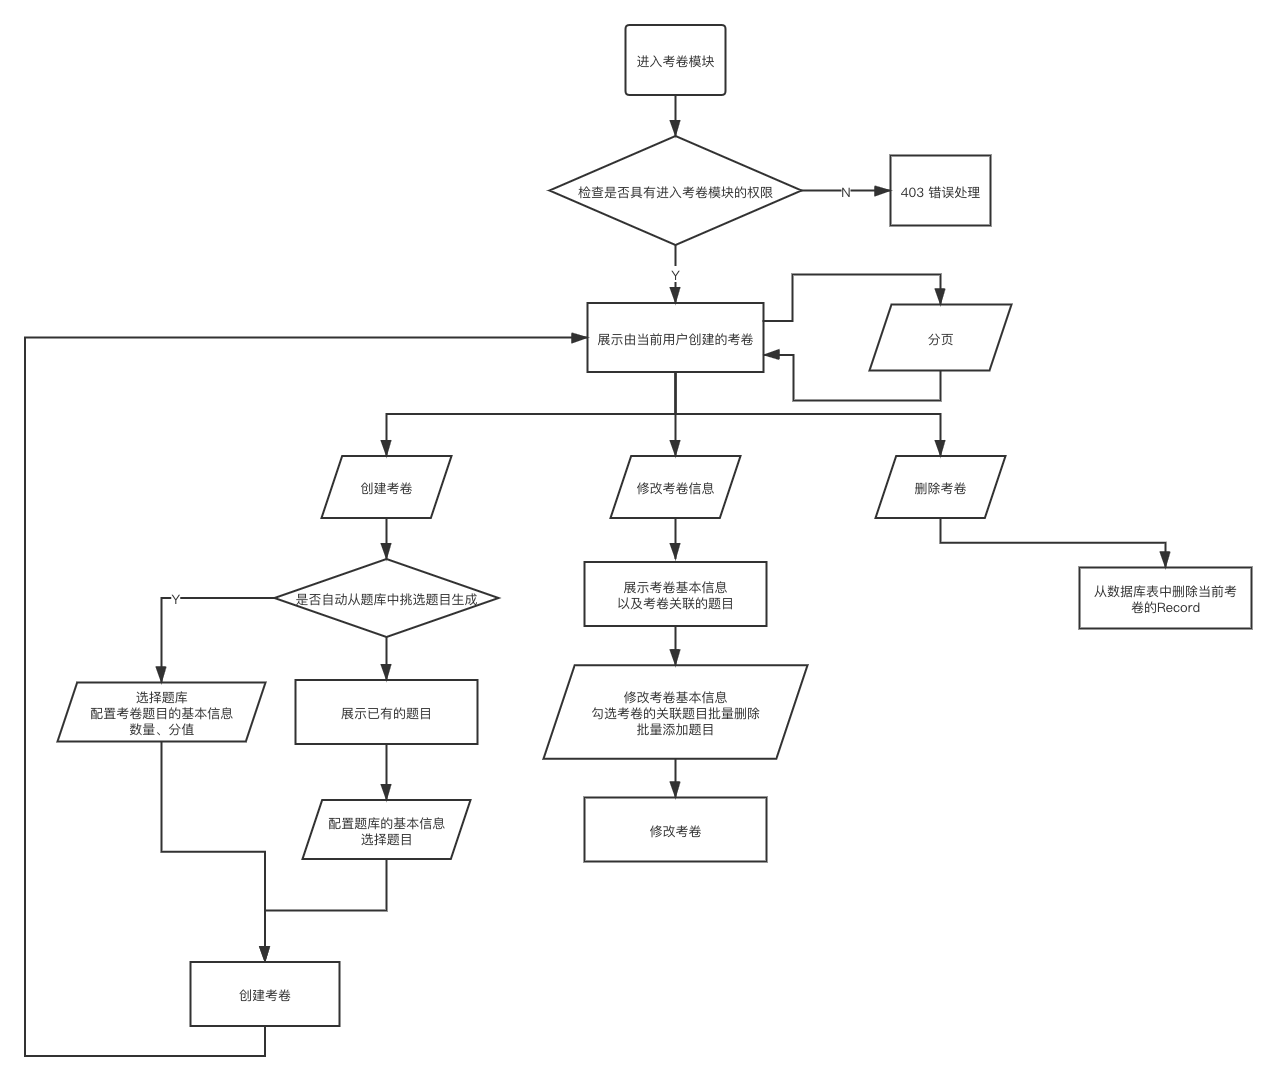
\includegraphics[width=\linewidth]{_images/考卷模块.png}
    \caption{考卷模块}
\end{figure}


\subsection{用户管理模块}
渲染用户模块前需要先检查是否有进入的权限,如果没有则需要一定的 403 反馈。正常操作流程下,没有权限是无法通过点击事件进入用户模块,但也可能通过浏览器的地址栏 URL,通过路由器强行渲染出对应的题库 View 组件,因此仍是需要在进入用户模块前进行权限检查。

进入用户模块后,以列表形式展示所有的用户。并可以通过 Select 框选择,按照不同的用户角色进行条件筛选,展示对应用户的情况。并且支持分页能力。

新增用户时需要填写用户的基本信息,并且需要选择用户的角色,赋予其权限划分。用户是通过 username 来区分的,所以在注册用户时,需要先判断 username 是否已存在,如果存在,则返回“用户名已存在”。如果不存在,将新用户信息添加到数据库。

修改用户和新增用户类似,也需要判断新的 username 是否已存在,如果不存在,则将修改后的信息更新到数据库。

删除用户仅仅将用户从 user 表中删除,而不删除所有相关联的其余表中的 creatorId(或将其设置为 -1)。这样就能保证其他原先创建的考卷、题库、题目,不会受到其创建人的用户被删除,而出现异常情况。其 creatorId 的失效也仅仅影响了查询部分。\upcite{ref7,ref22,ref17}

\begin{figure}[htb]
    \centering
    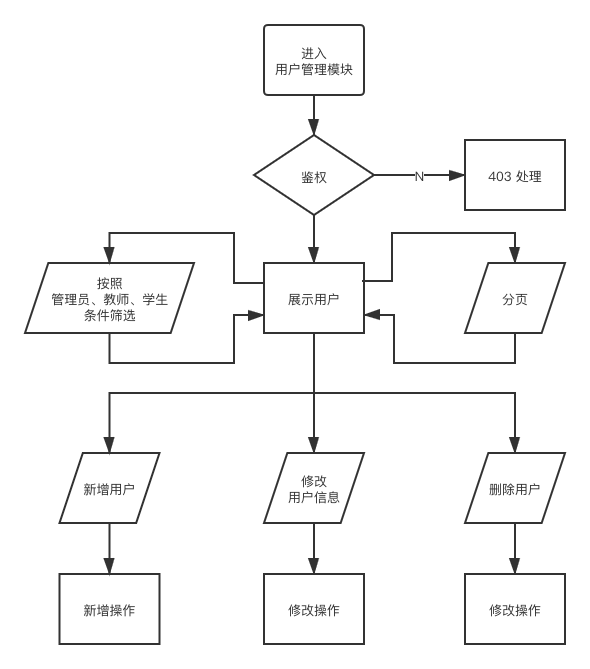
\includegraphics[width=0.7\linewidth]{_images/用户管理模块.png}
    \caption{用户管理模块}
\end{figure}


\subsection{考试模块}
所有的用户都有权限进入考试模块。首先展示的是所有的考试,所以在进入页面前会先请求所有的考试信息。
\begin{lstlisting}[language=JavaScript]
function getExamCardList() {
  return axios({
    url: api.ExamCardList,
    method: 'get',
    headers: {
      'Content-Type': 'application/json;charset=UTF-8'
    }
  })
}
\end{lstlisting}
\begin{lstlisting}[language=Java]
@GetMapping("/card/list")
@ApiOperation("获取考试列表,适配前端卡片列表")
ResultVO<List<ExamCardVo>> getExamCardList() {
    // 获取考试列表卡片
    ResultVO<List<ExamCardVo>> resultVO;
    try {
        List<ExamCardVo> examCardVoList = examService.getExamCardList();
        resultVO = new ResultVO<>(0, "获取考试列表卡片成功", examCardVoList);
    } catch (Exception e) {
        e.printStackTrace();
        resultVO = new ResultVO<>(-1, "获取考试列表卡片失败", null);
    }
    return resultVO;
}
\end{lstlisting}
其中,可以进行条件筛选。可以按照已结束的考试、参加过的考试、可参加的仍在有效时间内的、未开始的,进行对考试列表的筛选。如果是展示的参加过的考试,点击事件会展示考试的详情。包括考试的答案、问题的正确答案、正确答案的解析,以及考试的得分。

在考试列表中,可以选择考试参加。点击选择的考试将跳转到答题系统中,即可进行答题。答题过程中将会进行计时操作。提交答案前,将会进行检查是否有未作答的题目,如有则拒绝提交。提交考试后将跳转回考试模块的最初页面。

\begin{figure}[htb]
    \centering
    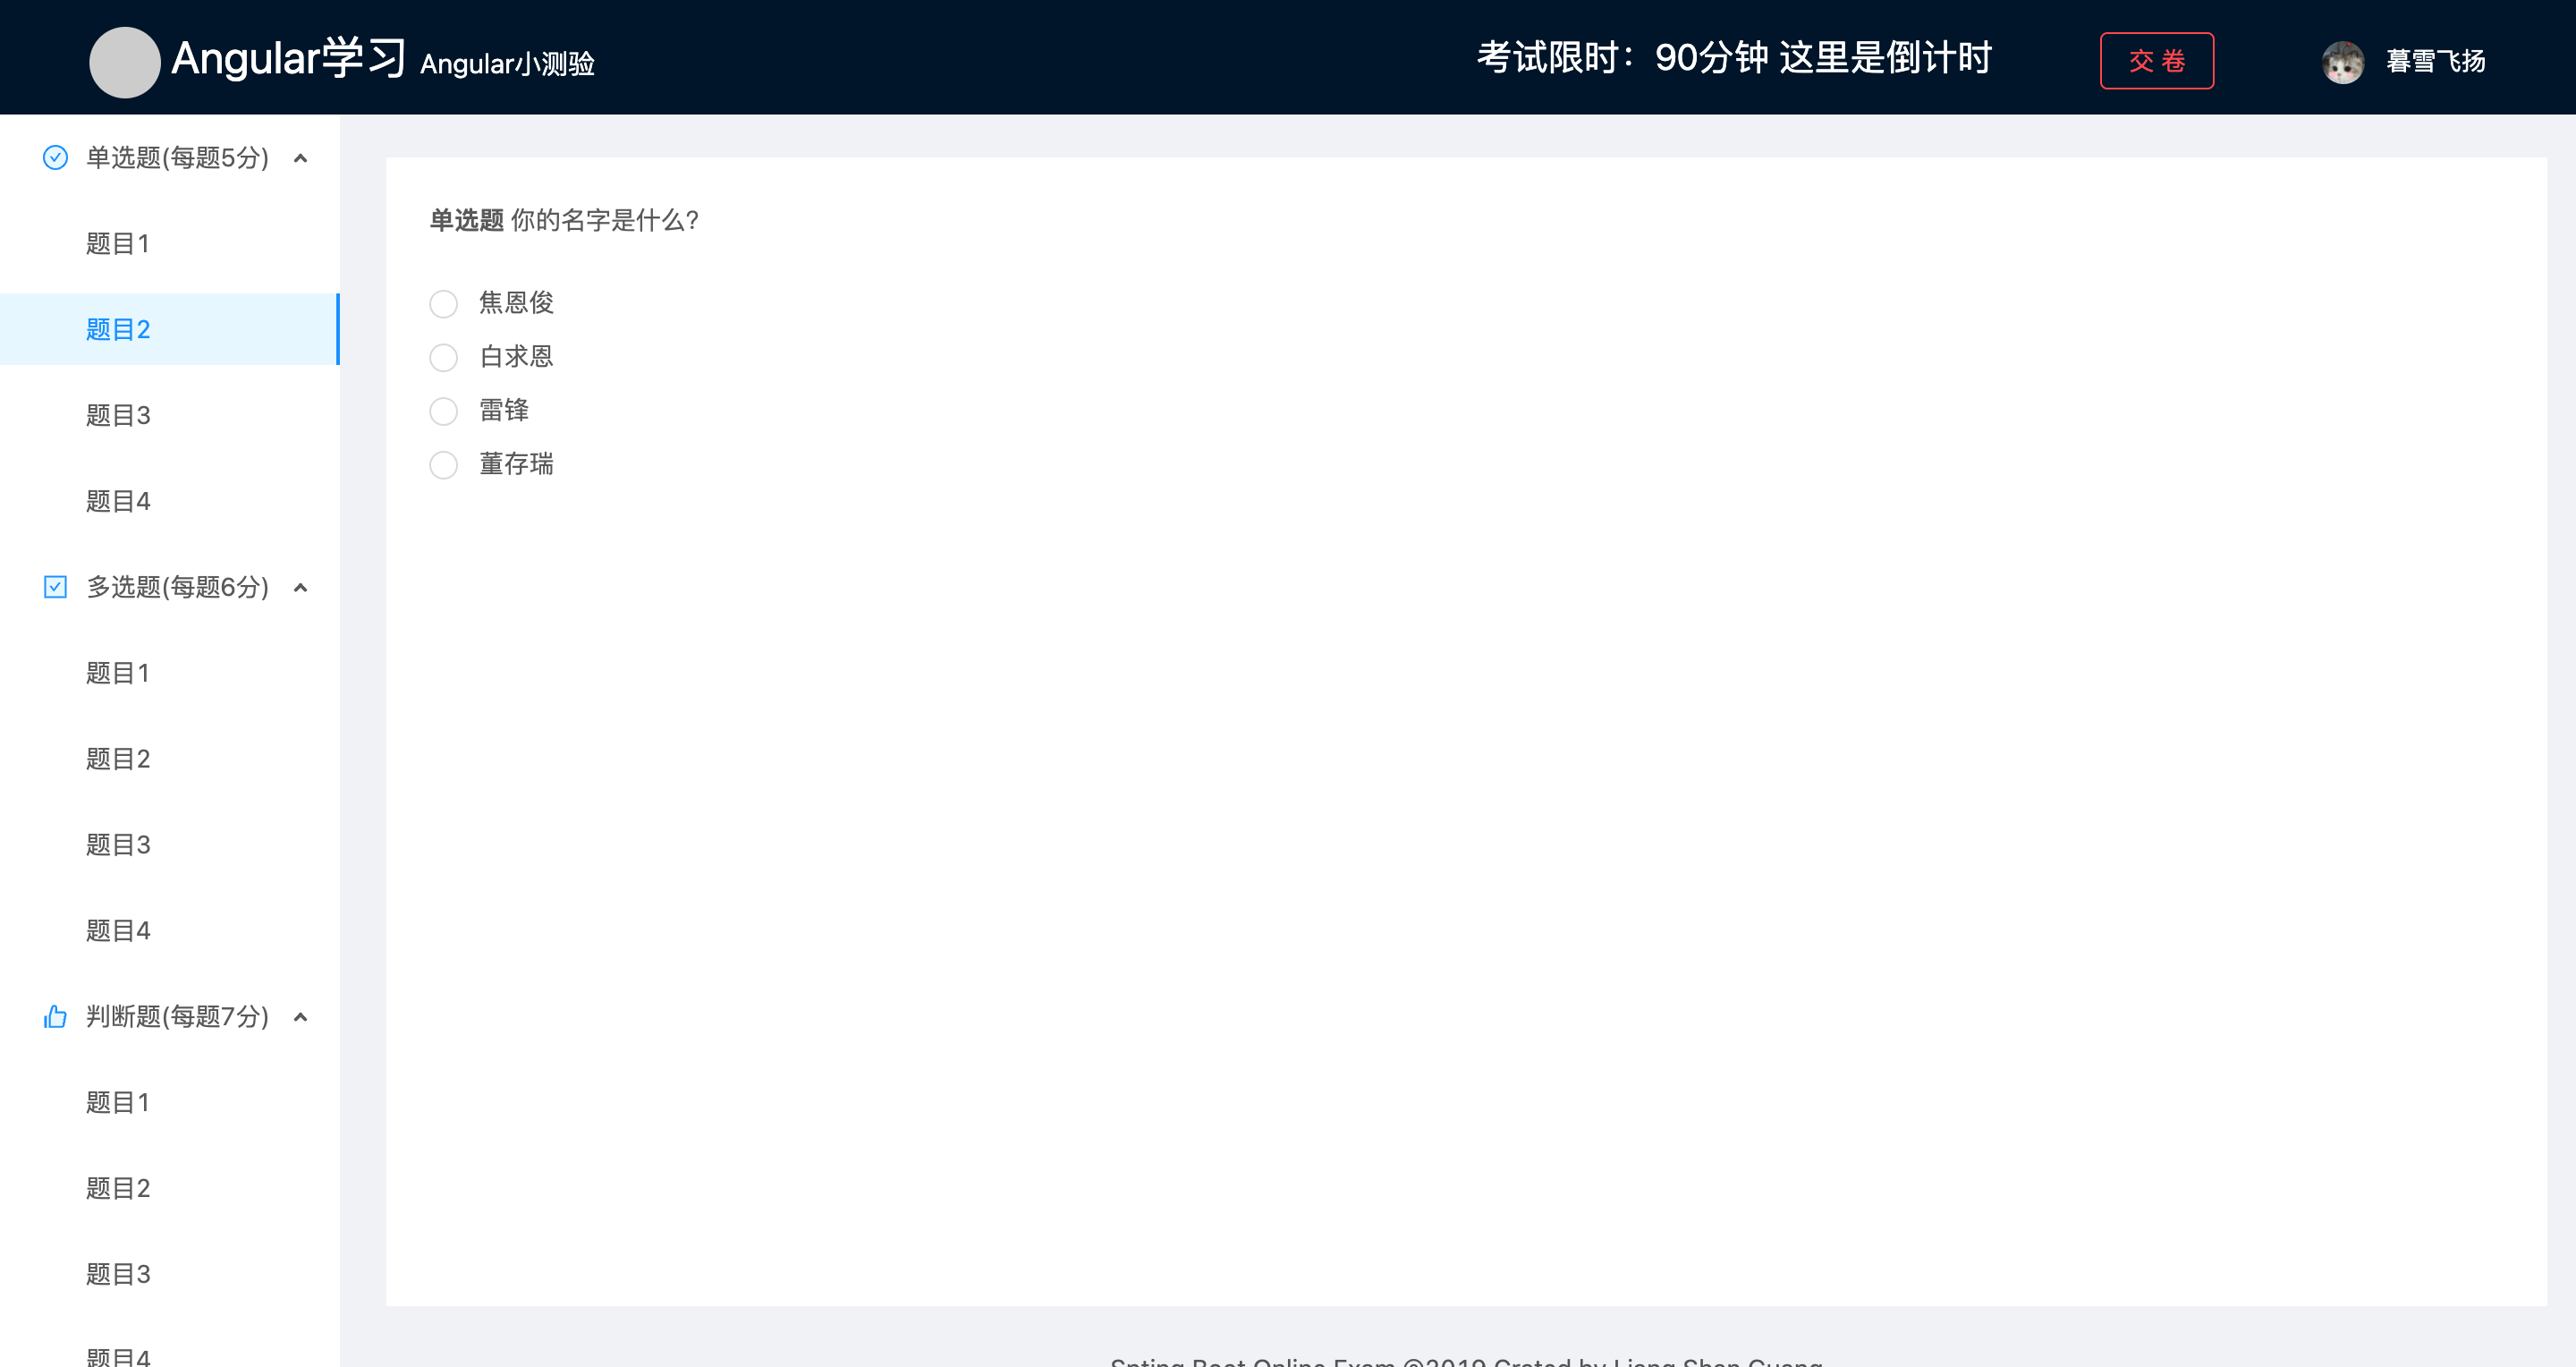
\includegraphics[width=\linewidth]{_images/答题系统.png}
    \caption{答题系统}
\end{figure}

创建考试并不是所有用户角色都拥有的权限。因而,创建考试的按钮需要根据当前登录的用户角色,通过 
\lstinline!v-if! 的方式决定是否渲染。点击创建考试,需要选择考试使用的考卷,以及填写考试的基本信息、起始时间、结束时间,以及时间限制。\upcite{ref18}

\begin{figure}[htb]
    \centering
    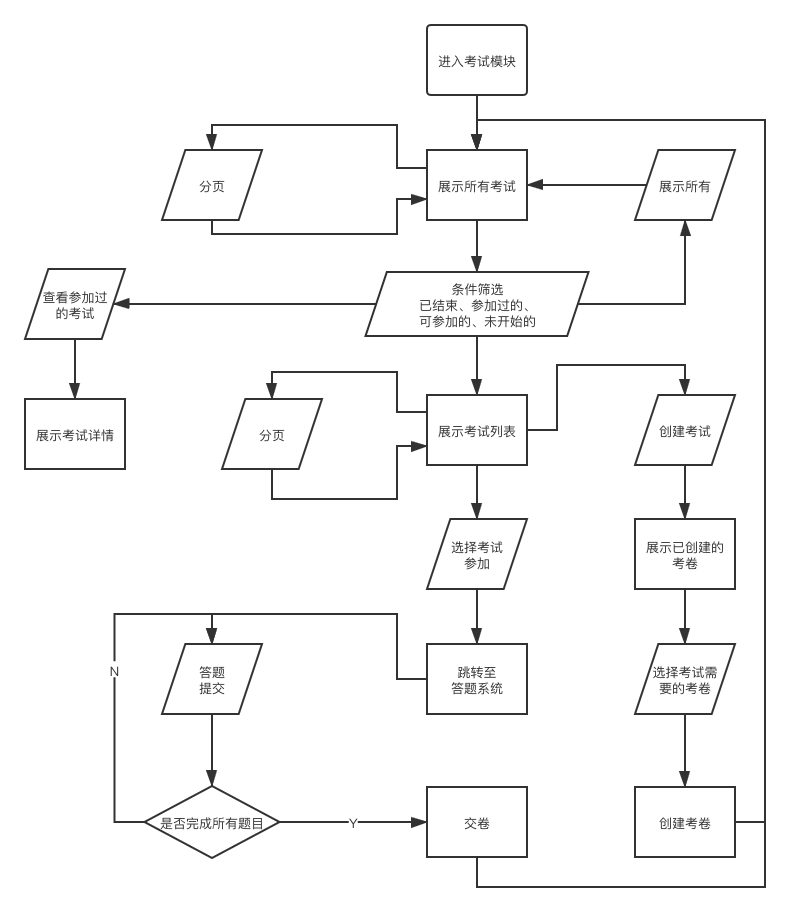
\includegraphics[width=\linewidth]{_images/考试模块.png}
    \caption{考试模块}
\end{figure}


